\chapter{Binomial Tree Method}
\label{sec:binomial-tree}

The \textit{binomial tree method} is a useful approach for pricing derivative instruments, including barrier options. It works by breaking down the time from the current moment (\(t = 0\)) to the option's maturity (\(T\)) into a finite number of steps (\(N\)). The more steps you use, the more accurate the price becomes, eventually converging to the theoretical option price.

\section{Binomial Tree Structure}

A binomial tree models the possible price movements of the underlying asset over time. At each step, the asset price can either go up or down. The price at any node in the tree is calculated using the formula:

\[
S_{i,j} = S_0 \cdot u^j \cdot d^{i-j}
\]

where:
\begin{itemize}
    \item \(S_{i,j}\) is the stock price at step \(i\), level \(j\),
    \item \(S_0\) is the initial stock price,
    \item \(u = e^{\sigma \sqrt{\Delta t}}\) is the up factor,
    \item \(d = \frac{1}{u}\) is the down factor,
    \item \(\Delta t = \frac{T}{N}\) is the time increment per step,
    \item \(\sigma\) is the volatility of the underlying asset.
\end{itemize}

The risk-neutral probabilities of an upward movement (\(p\)) and a downward movement (\(q\)) are:

\[
p = \frac{e^{r \Delta t} - d}{u - d}, \quad q = 1 - p
\]

where \(r\) is the risk-free interest rate.

\section{Example Calculation}

Let's consider an up-and-out European style put option with these parameters:
\(S_0 = 100\), \(B = 120\), \(K = 100\), \(r = 0.05\), \(T = 1\ \text{year}\), \(\sigma = 0.2\), \(N = 3\).

\begin{itemize}
    \item The time increment per step is:
    
    \[
    \Delta t = \frac{T}{N} = \frac{1}{3} \approx 0.3333 \, \text{years}
    \]

    \item The up and down factors are:
    
    \[
    u = e^{\sigma \sqrt{\Delta t}} = e^{0.2 \sqrt{0.3333}} \approx 1.1224, \quad d = \frac{1}{u} \approx 0.8909
    \]

    \item The risk-neutral probabilities are:
    
    \[
    p = \frac{e^{r \Delta t} - d}{u - d} = \frac{e^{0.05 \cdot 0.3333} - 0.8909}{1.1224 - 0.8909} \approx 0.5438, \\ q = 1 - p = 0.4562
    \]

    \item The payoff for an up-and-out European-style barrier put option at maturity is defined as:

    \[ 
    \text{Payoff} = 
    \begin{cases} 
    \max(K - S_T, 0), & \text{if } \max(S_t) < B \\ 
    0, & \text{if } \max(S_t) \geq B 
    \end{cases}
    \]

    where \(t \in [0, T]\).
    
\end{itemize}


\section{Tree Construction and Results}
\begin{figure}[h]
    \centering
    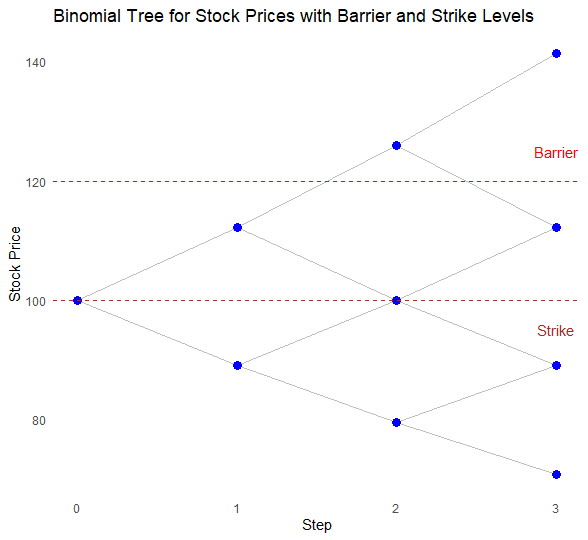
\includegraphics[width=.75\linewidth]{content/images/three-step.png}
    \caption{Binomial Tree with Barrier Level \(B = 120\) and Strike Price \(K = S_0\).}
    \label{fig:binomial-tree}
\end{figure}
Figure \ref{fig:binomial-tree} illustrates the binomial tree for the given parameters, showing the possible stock price movements and the resulting option values at each node. The calculated option price, considering the up-and-out barrier condition, is obtained through backward induction along the tree. This ensures that the barrier condition is applied at each step. The final option price using this method is 6.17. For reference, the actual option price using the analytical formula is 5.36.

\begin{figure}[h]
    \centering
    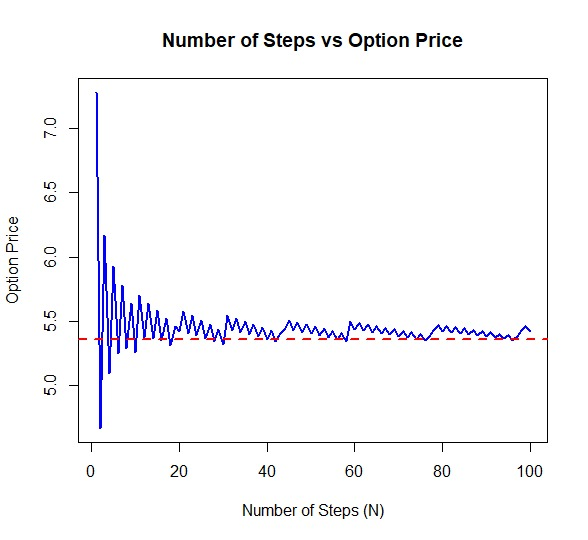
\includegraphics[width=.65\linewidth]{content/images/numstepsvsoptionprice.png}
    \caption{Option price converge to analytical solution as number of steps rise.}
    \label{fig:binom-nofsteps}
\end{figure}

The binomial tree method is great for pricing various options, including barrier options, because it's intuitive and systematic. As shown in Figure \ref{fig:binom-nofsteps}, the option price gets closer to the analytical solution as the number of steps (N) increases. However, this accuracy comes with higher computational complexity, especially for path-dependent options. In such cases, methods like Monte Carlo simulations or analytical approaches can be more efficient and scalable, providing accuracy without the heavy computational load. Balancing flexibility and efficiency is crucial when choosing the right pricing method for complex financial derivatives.